\documentclass[a4paper]{article}

%% Language and font encodings
\usepackage[english]{babel}
\usepackage[utf8]{inputenc}
\usepackage[T1]{fontenc}

%% Sets page size and margins
\usepackage[a4paper,top=3cm,bottom=2cm,left=3cm,right=3cm,marginparwidth=1.75cm]{geometry}
%\raggedright
\usepackage{caption}
\usepackage{subcaption}
\usepackage{amsmath,epsfig,graphicx,amsfonts}
\usepackage{booktabs}
\usepackage{multirow}
\begin{document}
\begin{figure}[!ht]
     \centering
     \begin{subfigure}{0.32\textwidth}
         \centering
         \caption*{$n=50, (|\mathcal{S}_\alpha|,|\mathcal{S}_\beta|)=(0,0)$}
         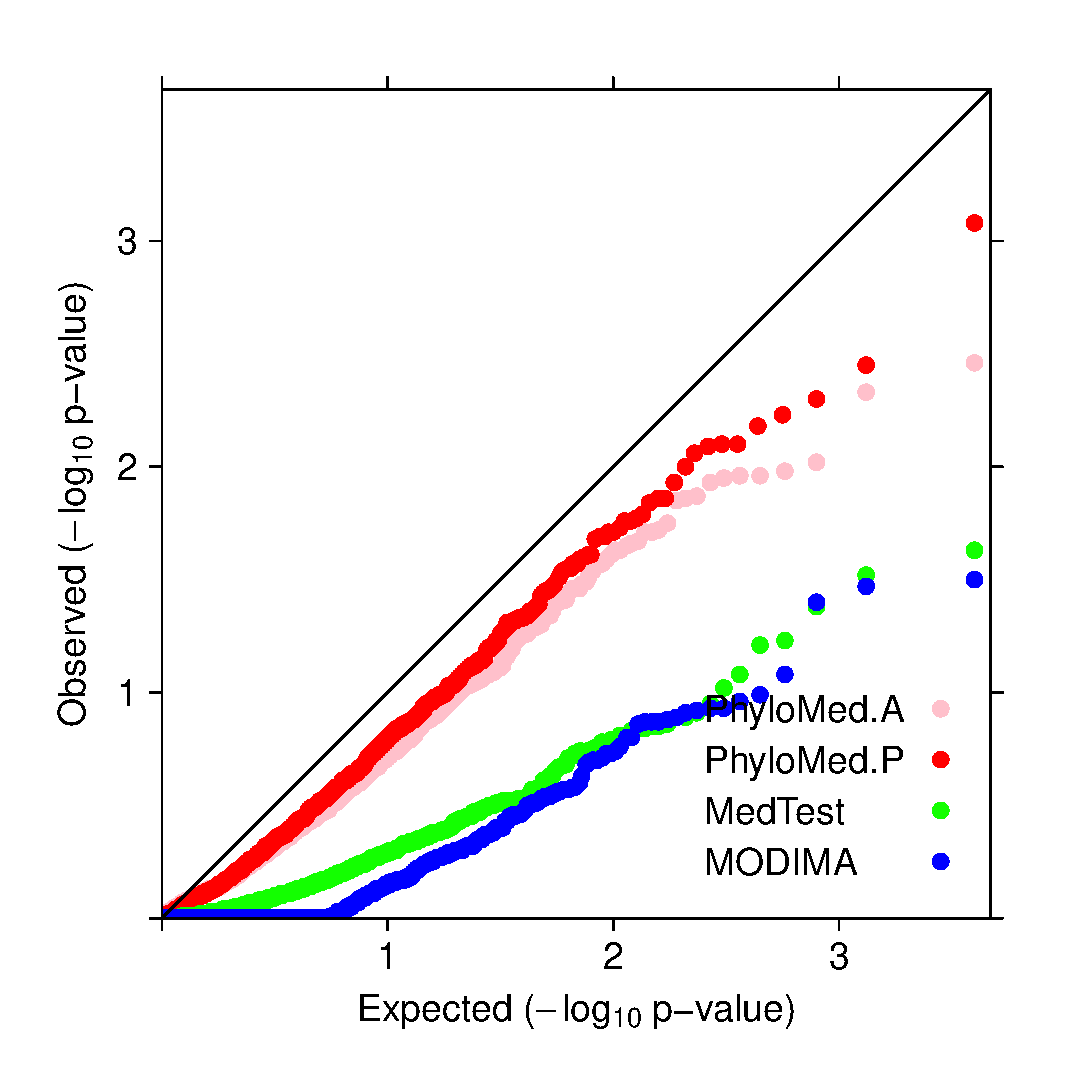
\includegraphics[width=\textwidth]{figure/qq_sscon00.eps}
     \end{subfigure}
     \hfill
     \begin{subfigure}{0.32\textwidth}
         \centering
         \caption*{$n=50, (|\mathcal{S}_\alpha|,|\mathcal{S}_\beta|)=(3 \text{ or } 6,0)$}
         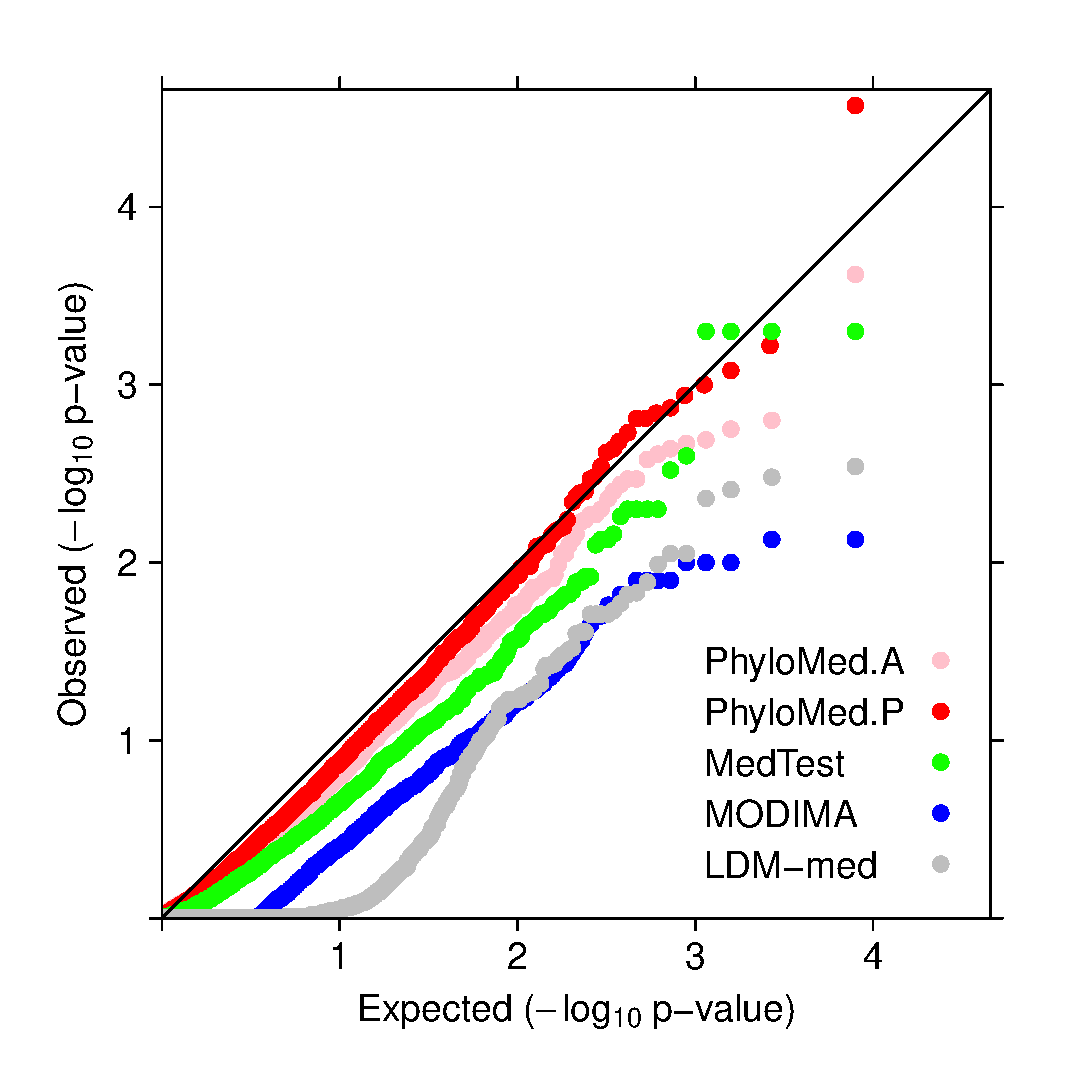
\includegraphics[width=\textwidth]{figure/qq_sscon10.eps}
     \end{subfigure}
     \hfill
     \begin{subfigure}{0.32\textwidth}
         \centering
         \caption*{$n=50, (|\mathcal{S}_\alpha|,|\mathcal{S}_\beta|)=(0, 3 \text{ or } 6)$}
         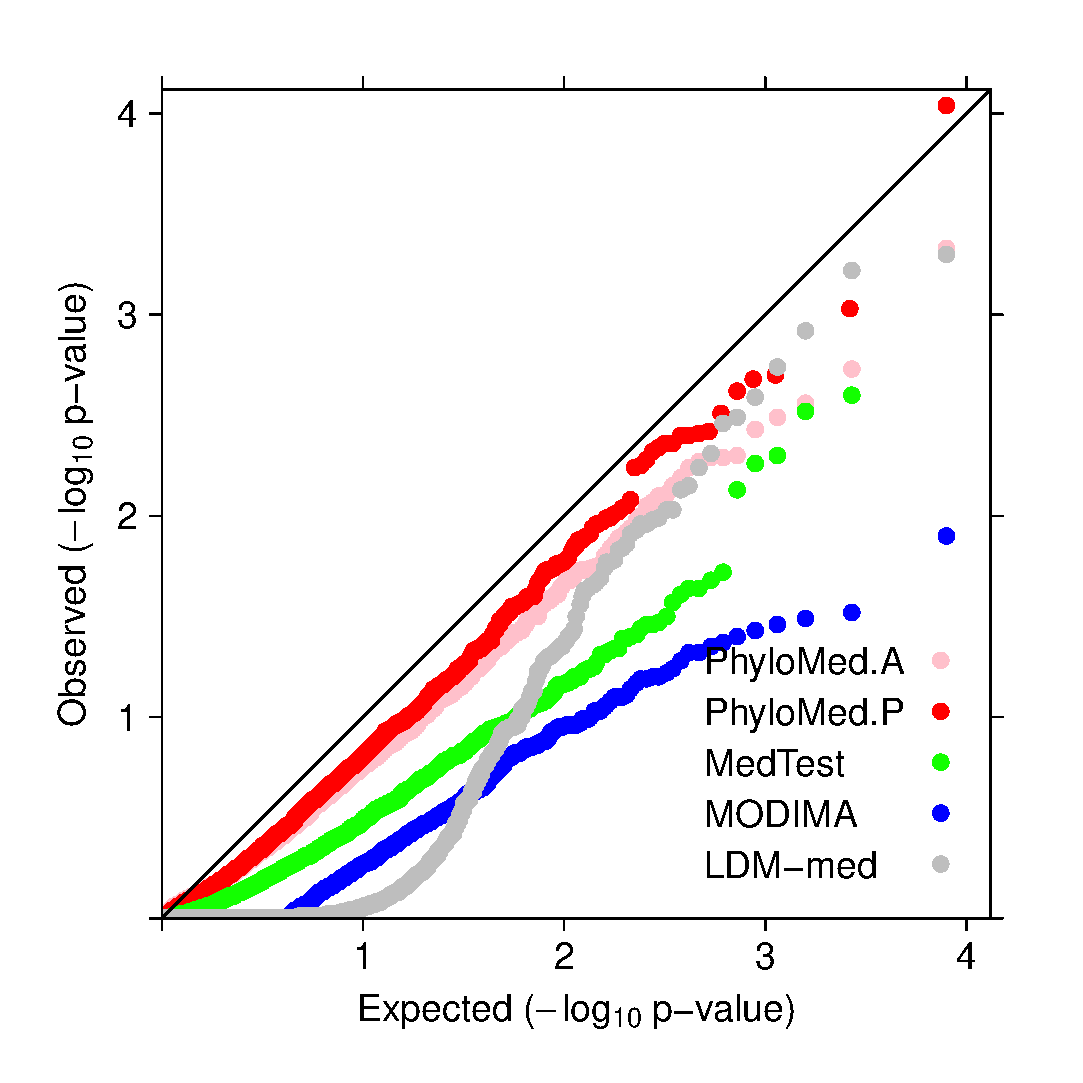
\includegraphics[width=\textwidth]{figure/qq_sscon01.eps}
     \end{subfigure}
     
     \begin{subfigure}{0.32\textwidth}
         \centering
         \caption*{$n=200, (|\mathcal{S}_\alpha|,|\mathcal{S}_\beta|)=(0,0)$}
         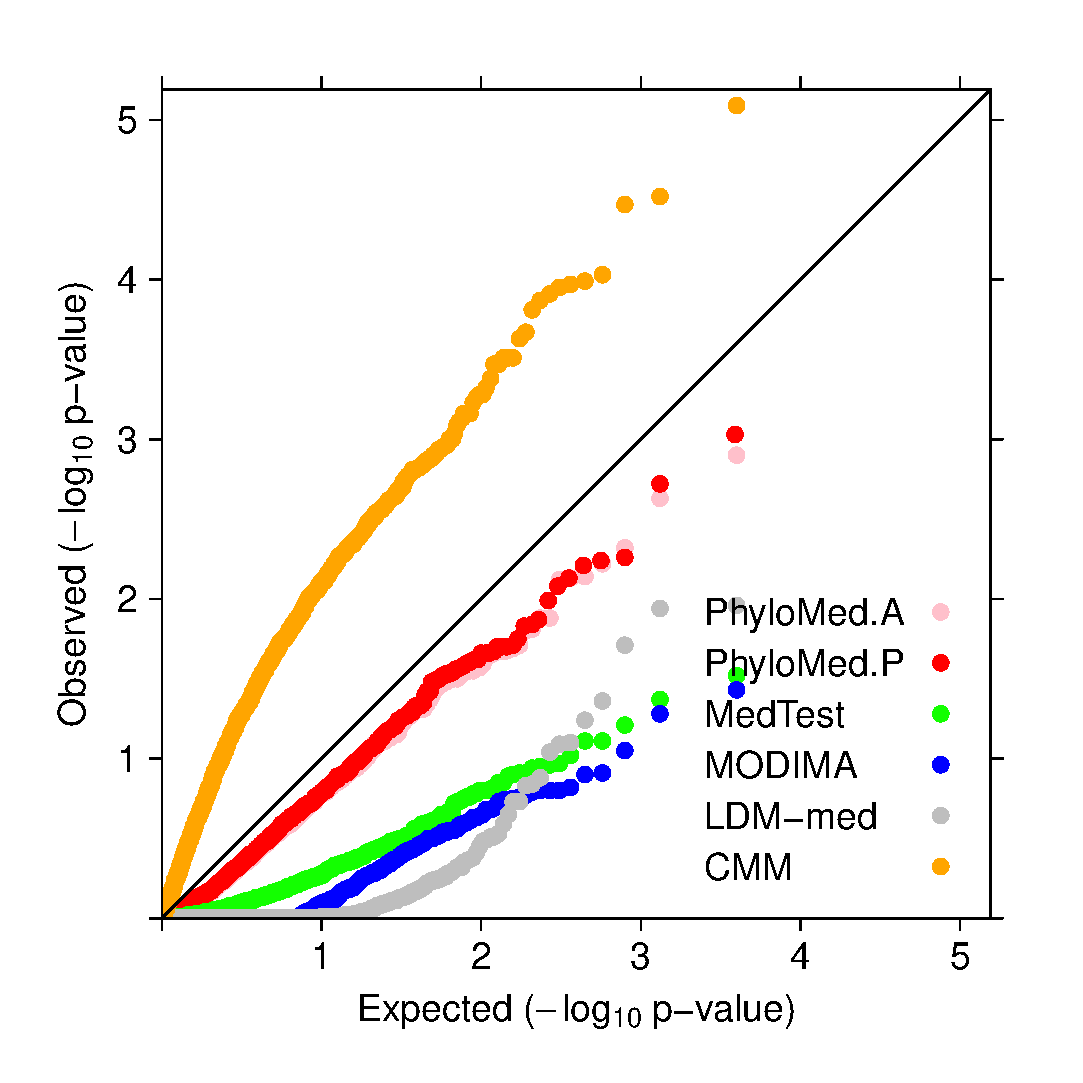
\includegraphics[width=\textwidth]{figure/qq_lscon00.eps}
     \end{subfigure}
     \hfill
     \begin{subfigure}{0.32\textwidth}
         \centering
         \caption*{$n=200, (|\mathcal{S}_\alpha|,|\mathcal{S}_\beta|)=(3 \text{ or } 6,0)$}
         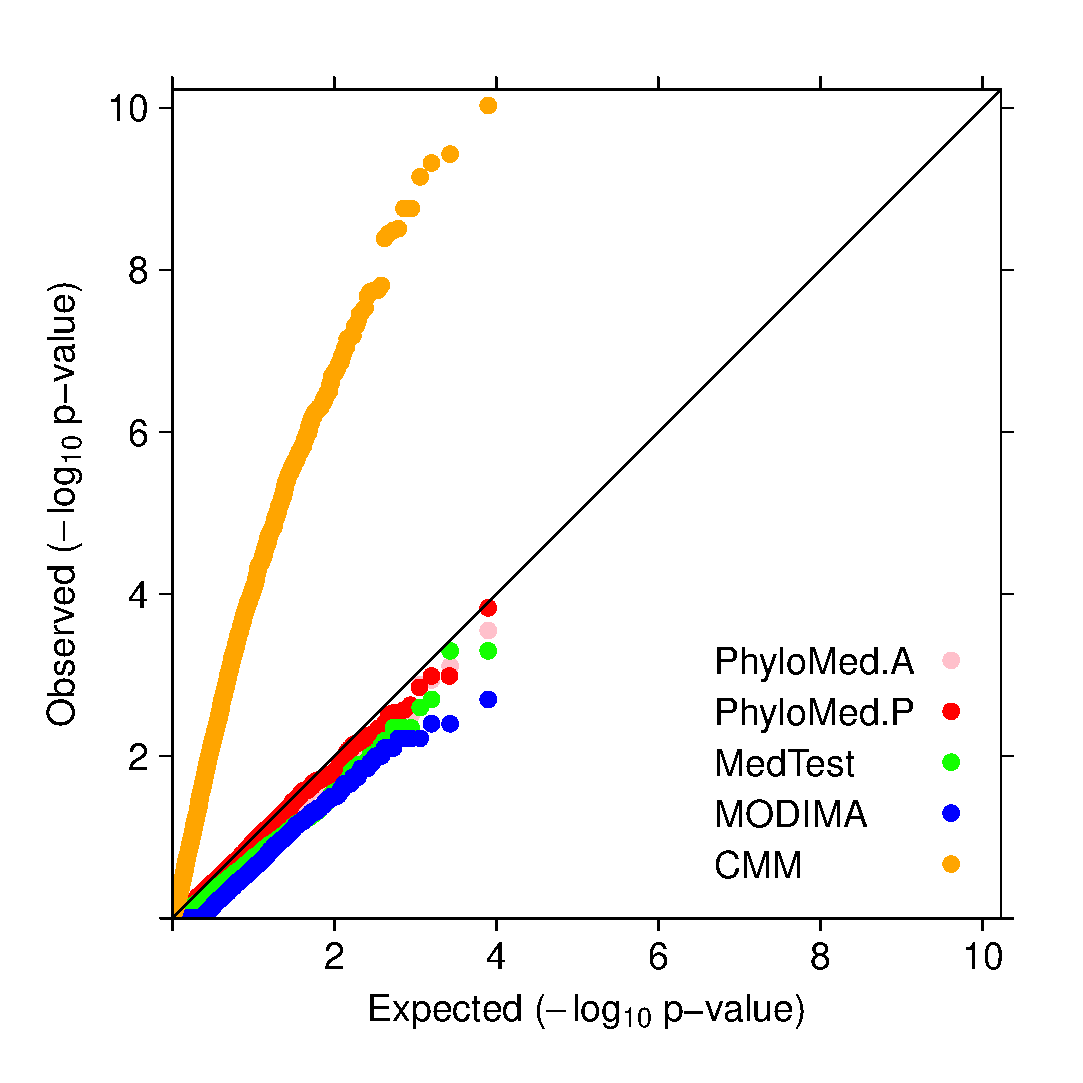
\includegraphics[width=\textwidth]{figure/qq_lscon10.eps}
     \end{subfigure}
     \hfill
     \begin{subfigure}{0.32\textwidth}
         \centering
         \caption*{$n=200, (|\mathcal{S}_\alpha|,|\mathcal{S}_\beta|)=(0, 3 \text{ or } 6)$}
         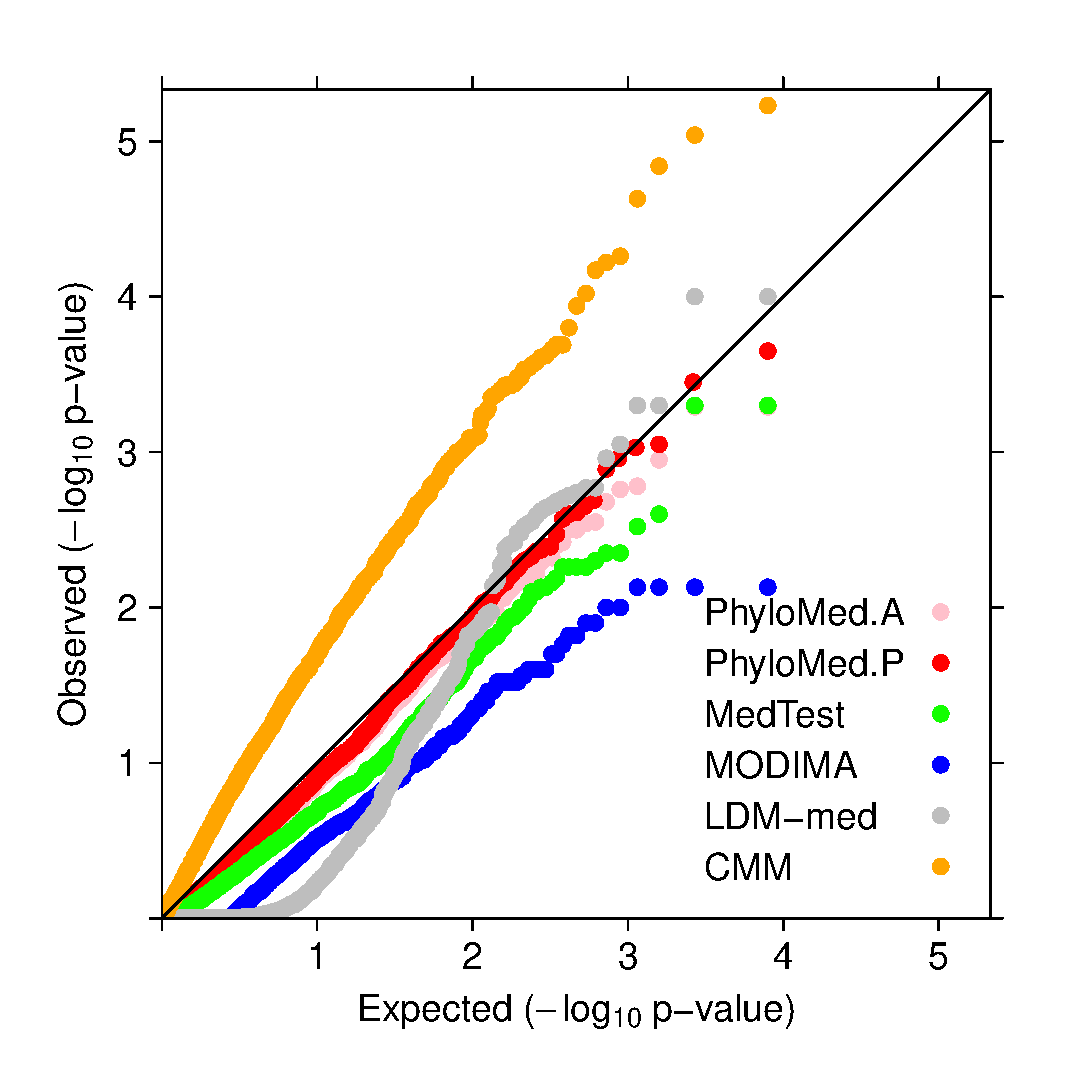
\includegraphics[width=\textwidth]{figure/qq_lscon01.eps}
     \end{subfigure}
\end{figure}
\thispagestyle{empty}
\newpage
\begin{figure}[!ht]
     \centering
     \begin{subfigure}{0.32\textwidth}
         \centering
         \caption*{$n=50, (|\mathcal{S}_\alpha|,|\mathcal{S}_\beta|)=(0,0)$}
         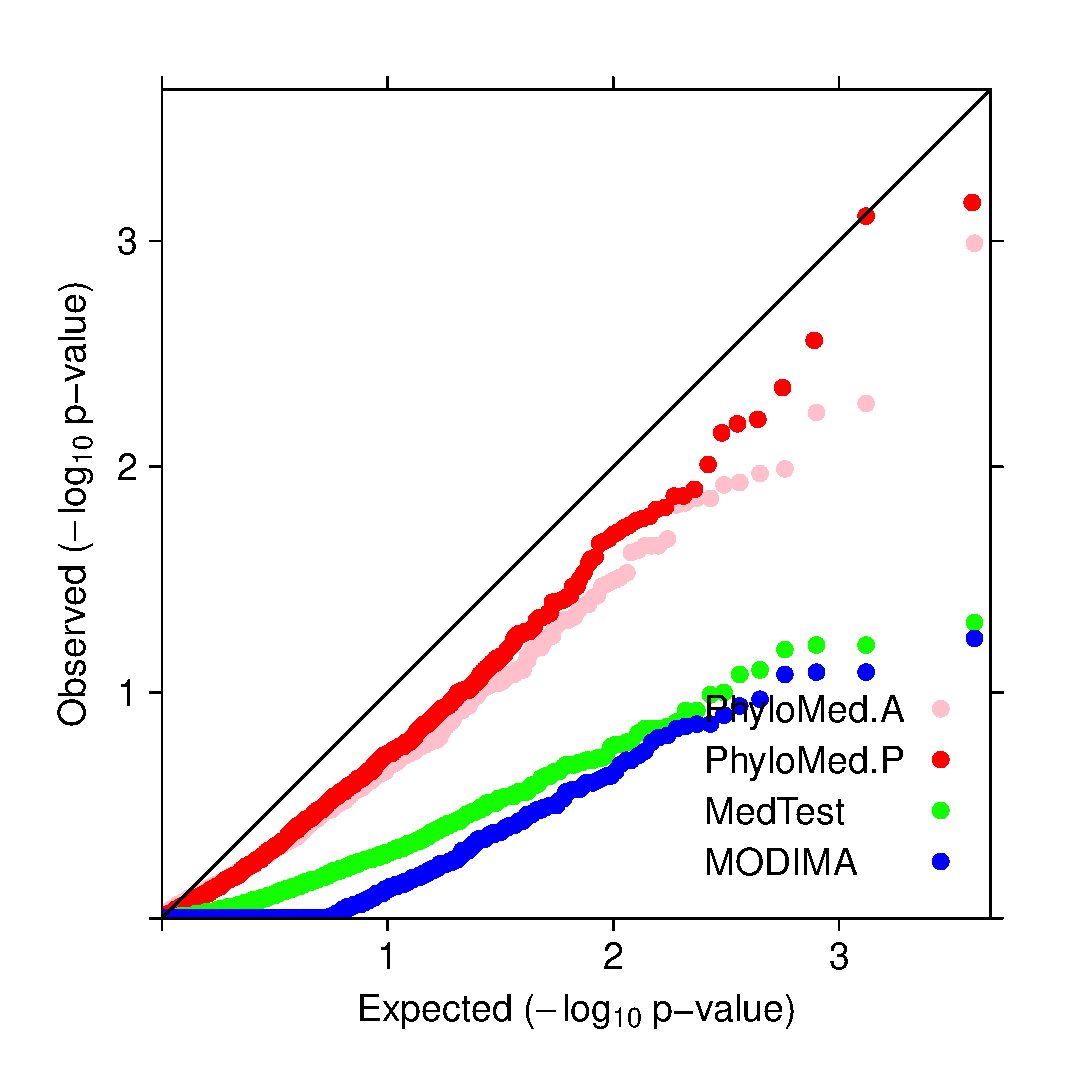
\includegraphics[width=\textwidth]{figure/qq_ssbin00.eps}
     \end{subfigure}
     \hfill
     \begin{subfigure}{0.32\textwidth}
         \centering
         \caption*{$n=50, (|\mathcal{S}_\alpha|,|\mathcal{S}_\beta|)=(3 \text{ or } 6,0)$}
         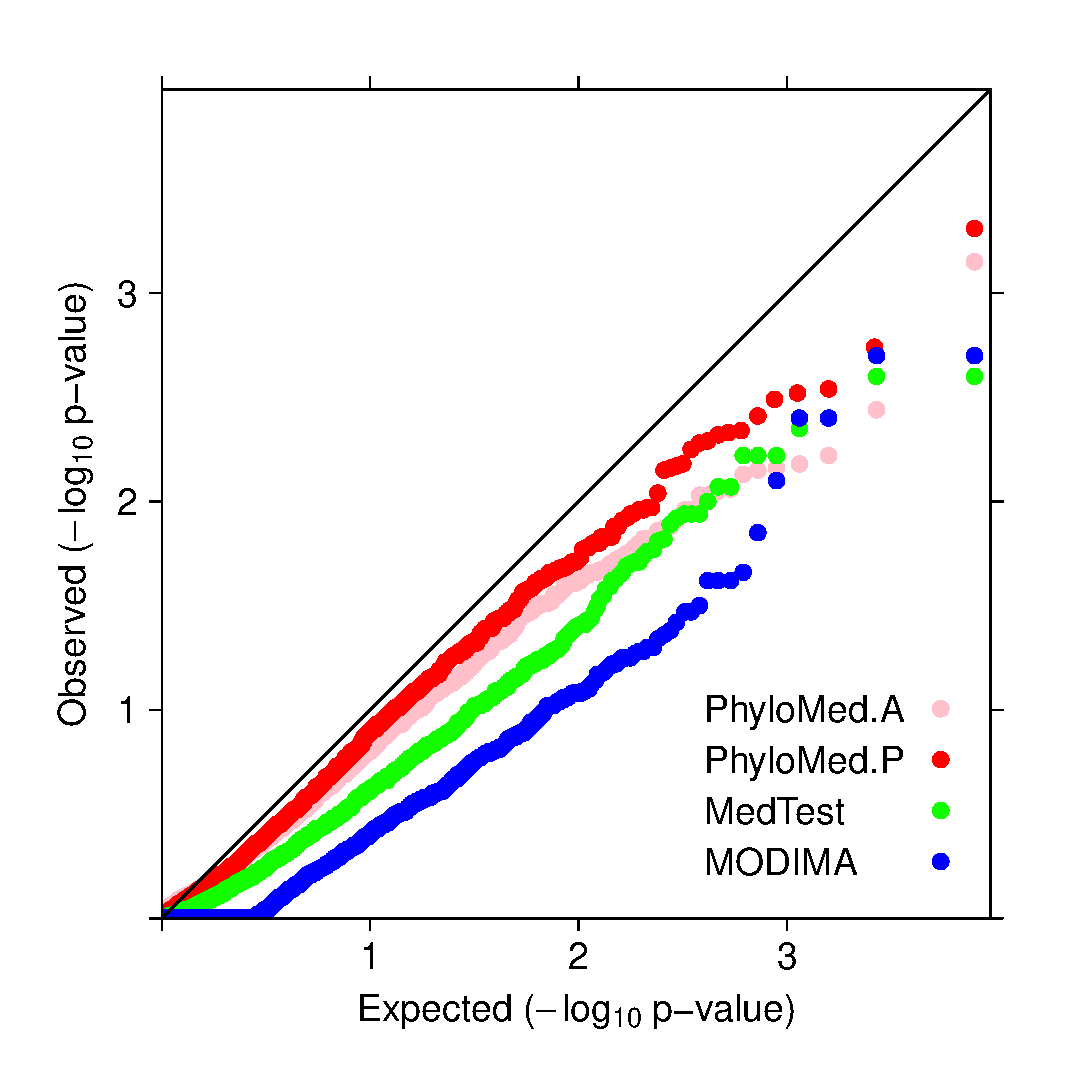
\includegraphics[width=\textwidth]{figure/qq_ssbin10.eps}
     \end{subfigure}
     \hfill
     \begin{subfigure}{0.32\textwidth}
         \centering
         \caption*{$n=50, (|\mathcal{S}_\alpha|,|\mathcal{S}_\beta|)=(0, 3 \text{ or } 6)$}
         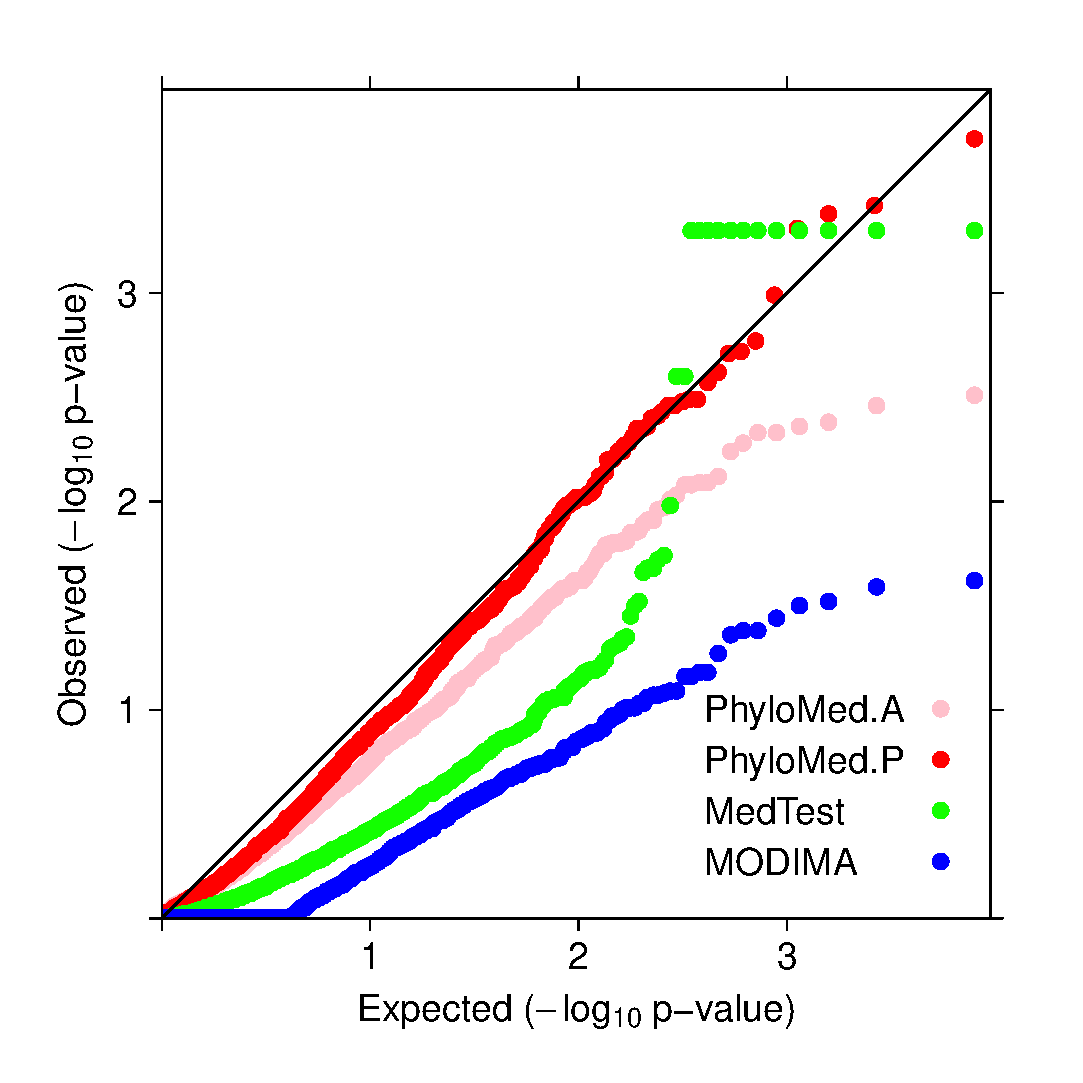
\includegraphics[width=\textwidth]{figure/qq_ssbin01.eps}
     \end{subfigure}
     
     \begin{subfigure}{0.32\textwidth}
         \centering
         \caption*{$n=200, (|\mathcal{S}_\alpha|,|\mathcal{S}_\beta|)=(0,0)$}
         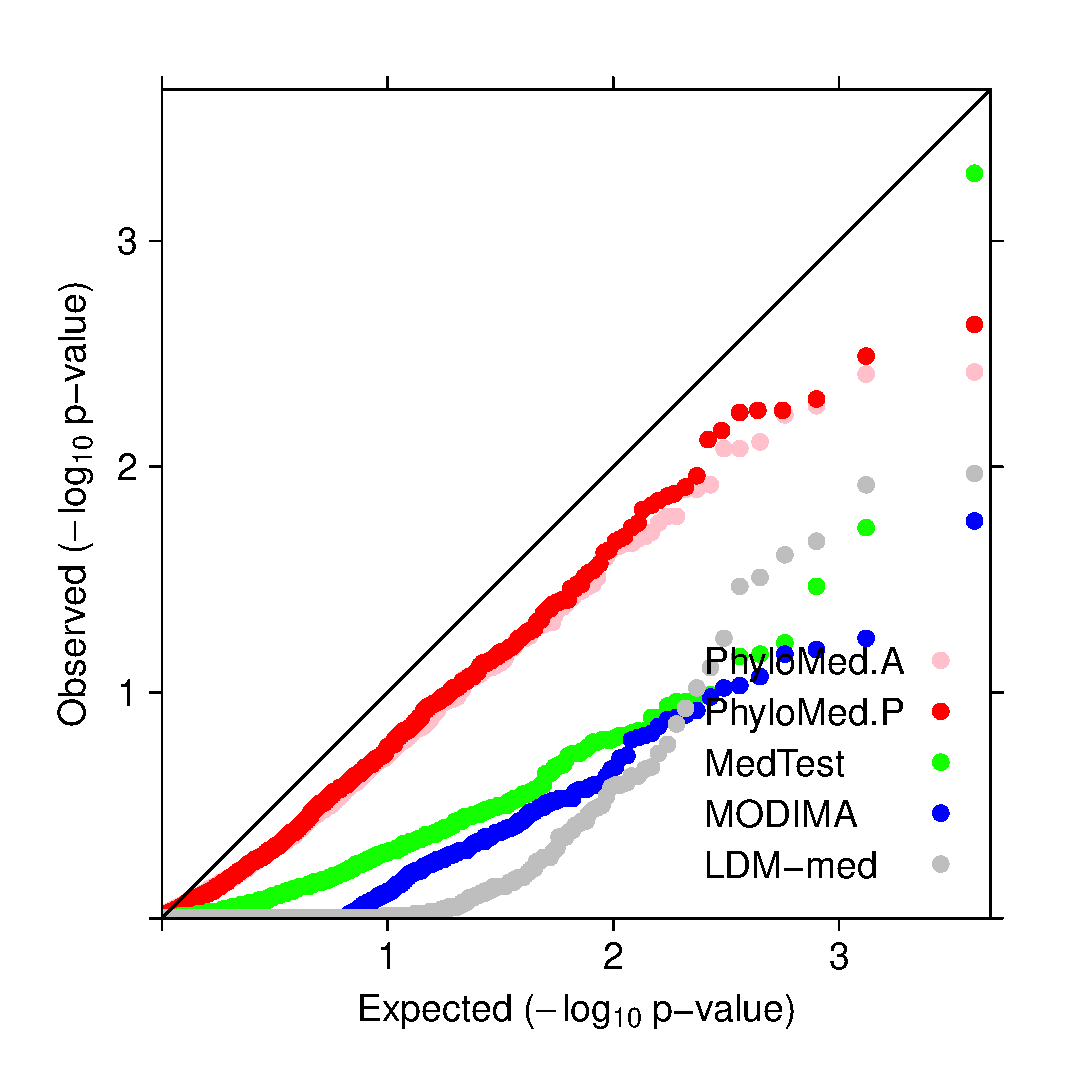
\includegraphics[width=\textwidth]{figure/qq_lsbin00.eps}
     \end{subfigure}
     \hfill
     \begin{subfigure}{0.32\textwidth}
         \centering
         \caption*{$n=200, (|\mathcal{S}_\alpha|,|\mathcal{S}_\beta|)=(3 \text{ or } 6,0)$}
         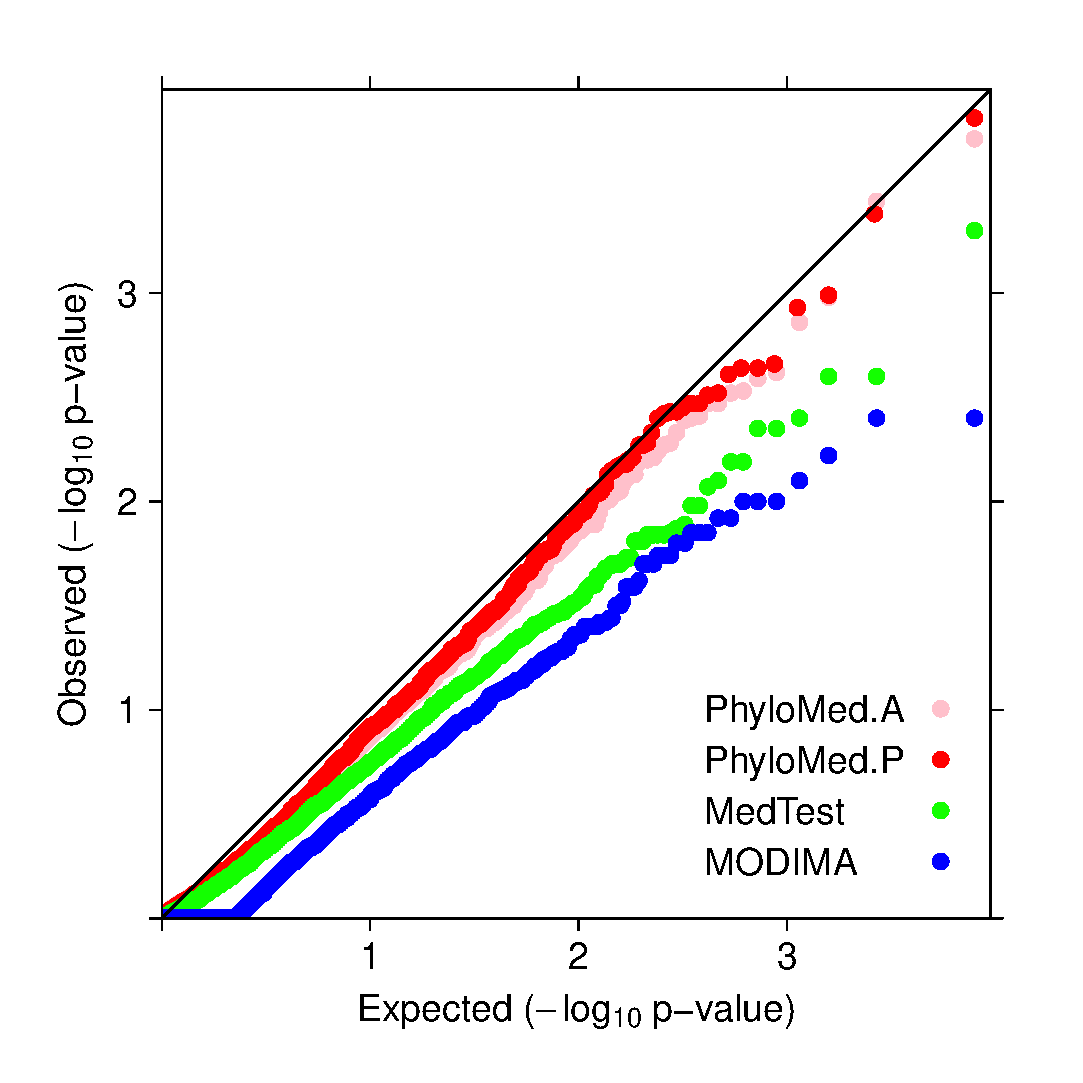
\includegraphics[width=\textwidth]{figure/qq_lsbin10.eps}
     \end{subfigure}
     \hfill
     \begin{subfigure}{0.32\textwidth}
         \centering
         \caption*{$n=200, (|\mathcal{S}_\alpha|,|\mathcal{S}_\beta|)=(0, 3 \text{ or } 6)$}
         \includegraphics[width=\textwidth]{figure/qq_lsbin01.eps}
     \end{subfigure}
\end{figure}
\thispagestyle{empty}
\newpage
\begin{figure}[!ht]
     \centering
     \begin{subfigure}{0.32\textwidth}
         \centering
         \caption*{$n=200, (|\mathcal{S}_\alpha|,|\mathcal{S}_\beta|)=(0,0)$}
         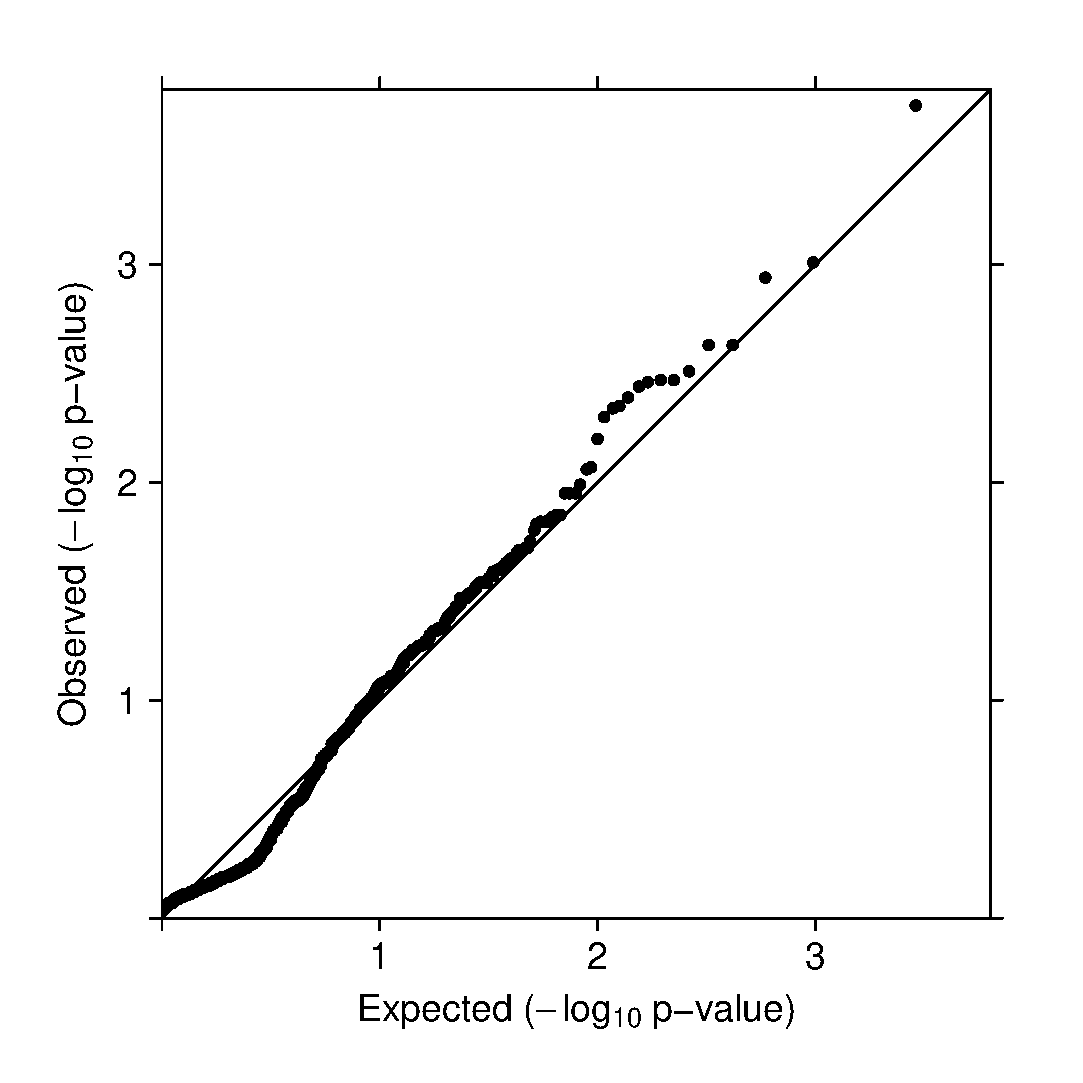
\includegraphics[width=\textwidth]{figure/qq_dact00.eps}
     \end{subfigure}
     \hfill
     \begin{subfigure}{0.32\textwidth}
         \centering
         \caption*{$n=200, (|\mathcal{S}_\alpha|,|\mathcal{S}_\beta|)=(3 \text{ or } 6,0)$}
         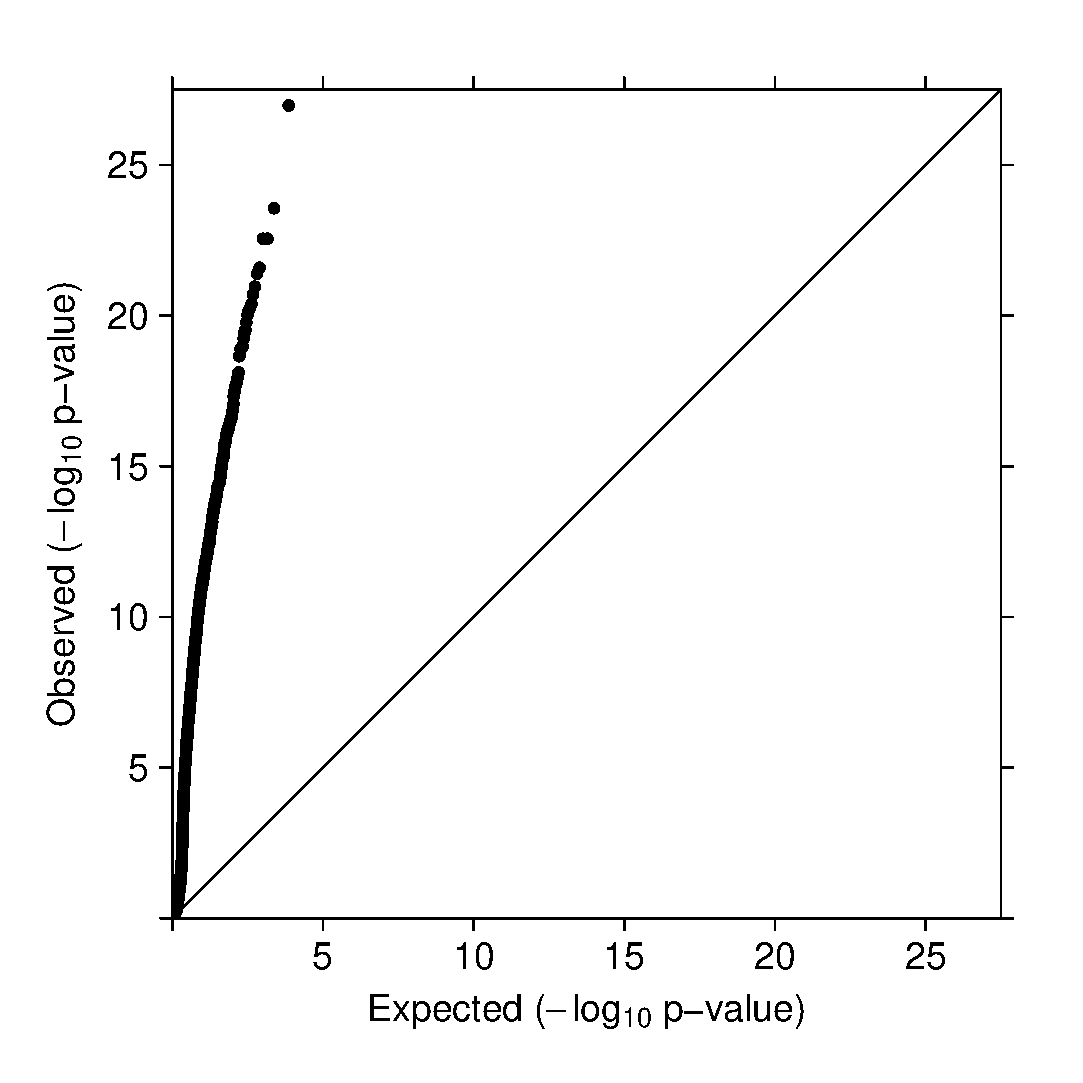
\includegraphics[width=\textwidth]{figure/qq_dact10.eps}
     \end{subfigure}
     \hfill
     \begin{subfigure}{0.32\textwidth}
         \centering
         \caption*{$n=200, (|\mathcal{S}_\alpha|,|\mathcal{S}_\beta|)=(0, 3 \text{ or } 6)$}
         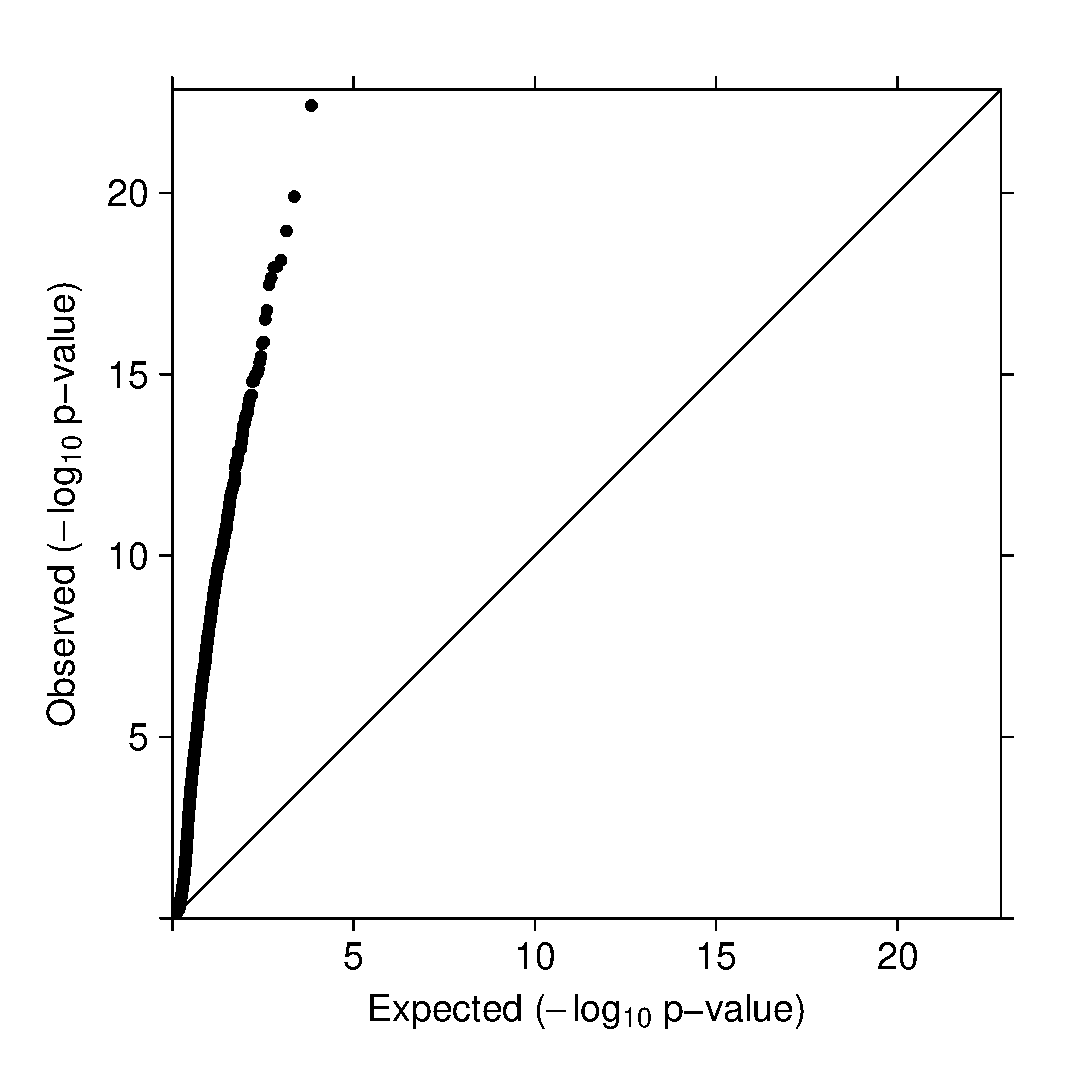
\includegraphics[width=\textwidth]{figure/qq_dact01.eps}
     \end{subfigure}
\end{figure}

\thispagestyle{empty}
\newpage
\captionsetup[subfigure]{position=top, labelfont=bf,labelformat=simple,textfont=normalfont,singlelinecheck=off,justification=raggedright}
\renewcommand{\thesubfigure}{\alph{subfigure}}
\begin{figure}[!ht]
    \centering
    
    \begin{subfigure}{0.66\textwidth}
    \caption{}
    \centering
    \includegraphics[width=\textwidth]{figure/Cecal.tree.pdf}
    \end{subfigure}
    \hfill
    \begin{subfigure}{0.33\textwidth}
    \caption{}
    \centering
    \includegraphics[width=\textwidth]{figure/Cecal.qqplot.pdf}
    \end{subfigure}
    \hfill
    \begin{subfigure}{0.66\textwidth}
    \caption{}
    \centering
    \includegraphics[width=\textwidth]{figure/Cecal.boxscatter.pdf}
    \end{subfigure}
    \hfill
    \begin{subfigure}{0.33\textwidth}
    \caption{}
    \centering
    \includegraphics[width=\textwidth]{figure/Cecal.subtreeWlink.png}
    \end{subfigure}
\end{figure}
\thispagestyle{empty}

\end{document}

